\section*{Introduction}
This report explores the implementation of a queue data structure using a fixed-size array and discusses the wrap-around technique, which addresses the limitations typically associated with array-based queues. A queue is a fundamental data structure that follows the First-In-First-Out (FIFO) principle, where elements are added at the rear and removed from the front. While linked lists are commonly used to implement queues due to their dynamic nature, they require frequent memory allocation and deallocation, which can be inefficient in terms of memory usage. In contrast, an array-based queue offers better memory utilization but faces challenges when elements are removed from the front or when the array becomes full. The wrap-around technique provides an elegant solution to these challenges by allowing the queue to reuse space efficiently.

\section*{Method}
The implementation utilized standard C libraries, including \texttt{stdlib.h}, \texttt{stdio.h}, \texttt{time.h}, and \texttt{limits.h}. Measurements were conducted on an Intel i7-13700K CPU with default frequency settings. The code was compiled using GCC without optimizations (\texttt{-O0}). Code from previous labs was used to conduct the benchmark. The benchmark methodology includes random generation of array elements, 50 iterations to obtain reliable average measurements, and time measurements in nanoseconds using \texttt{clock_gettime()}. The internet tool "mycurvefit.com" was used to find the best-fit function for the data.

\section*{Hypothesis}
The wrap-around technique allows the queue to "wrap around" the array, effectively reusing the space occupied by removed elements. This report presents the implementation of a wrap-around queue, analyzes its performance, and compares it with other queue implementations. The hypothesis is that the wrap-around queue will demonstrate improved performance in terms of time complexity compared to a standard array-based queue, particularly when dealing with large numbers of enqueue and dequeue operations. The wrap-around technique should enable constant-time operations, $O(1)$, regardless of the size of the queue or the number of elements added or removed.

\section*{Implementation}
\begin{figure}
    \centering
    \includegraphics[width=0.5\textwidth]{IMG_20211006_0001.jpg}
    \caption{Illustration of the logic of the wrap implementation}
    \label{fig:wrap_illustration}
\end{figure}
In this section, the key components of the wrap-around queue implementation are explained. The implementation involves creating a queue structure, enqueueing elements, extending the queue when necessary, and dequeueing elements. Each of these operations is designed to ensure efficient memory usage and constant-time performance.

\subsection*{Code Review}
\subsubsection*{Structure of Wrap Queue}
\begin{minted}{c}
    typedef struct queue {
        int arraySize;
        int *list;
        int firstIndex;
        int lastIndex;
        int count;        
    } queue;

    queue *create_queue(int arraySize) {
        queue *q = (queue*)malloc(sizeof(queue));
        int *list = (int *)malloc(arraySize * sizeof(int));
        q->arraySize = arraySize;
        q->list = list;
        q->firstIndex = 0;
        q->lastIndex = 0;
        q->count = 0;
        return q;
    }
\end{minted}
The first step in implementing the wrap-around queue is to define its structure. The structure includes the size of the array, a pointer to the array, indices for the front and rear of the queue, and a count of the elements currently in the queue. A function is then created to initialize the queue, allocating memory for the array and setting the initial values of the indices and count. The time complexity of this initialization function is $O(1)$.

\subsubsection*{Enqueue a Number to the Queue}
\begin{minted}{c}
    void enque(queue* q, int v) {
        if (q->count == q->arraySize) {
            extendQueue(q);
        }
        
        q->list[q->lastIndex] = v;
        q->lastIndex = (q->lastIndex + 1) % q->arraySize; 
        q->count++;
    }
\end{minted}
The enqueue function adds an element to the rear of the queue. If the queue is full, the function extends the array to accommodate more elements. The rear index is updated using the wrap-around technique, ensuring that it cycles back to the beginning of the array when it reaches the end. The time complexity of the enqueue function is $O(1)$ under normal conditions, but it becomes $O(n)$ when the array needs to be extended.

\subsubsection*{Extend the Queue}
\begin{minted}{c}
    void extendQueue(queue *q) {
        int *biggerList = (int *)malloc(q->arraySize * 2 * sizeof(int));
        
        for (int i = 0; i < q->count; i++) {
            int oldIndex = (q->firstIndex + i) % q->arraySize;
            biggerList[i] = q->list[oldIndex];
        }
        
        free(q->list);
        q->list = biggerList;
        q->firstIndex = 0;  
        q->lastIndex = q->count;  
        q->arraySize = q->arraySize * 2;
    }
\end{minted}
The extendQueue function doubles the size of the array when the queue becomes full. It copies the existing elements to the new array, ensuring that the order is preserved. The front and rear indices are adjusted to reflect the new array size. The time complexity of this function is $O(n)$, as it involves copying all elements from the old array to the new one.

\subsubsection*{Dequeue a Number from the Queue}
\begin{minted}{c}
    int dequeue(queue *q) {
        int res = 0;
        if (q->count > 0) { 
            res = q->list[q->firstIndex];
            q->firstIndex++;
            q->count--;
            if (q->firstIndex >= q->arraySize) {
                q->firstIndex = 0;
            }
        }
        return res;
    }
\end{minted}
The dequeue function removes an element from the front of the queue and returns its value. The front index is incremented, and if it exceeds the array size, it wraps around to the beginning. The time complexity of this function is $O(1)$, as it involves simple index manipulation and does not require traversing the array.

\section*{Performance and Analysis}
\subsection*{Performance}
\section*{Performance and Analysis}
\subsection*{Performance}
\begin{table}[h]
    \centering
    \begin{tabular}{|l|c|c|c|c|}
    \hline
    \textbf{Size} & \textbf{Min (µs)} & \textbf{Max (µs)} & \textbf{Avg (µs)} & \textbf{Avg/op (ns)} \\
    \hline
    1000 & 39.12 & 49.85 & 39.59 & 39.59 \\
    2000 & 20.37 & 88.76 & 23.06 & 11.53 \\
    4000 & 40.57 & 48.46 & 41.14 & 10.28 \\
    8000 & 63.53 & 125.07 & 86.19 & 10.77 \\
    16000 & 135.28 & 326.90 & 159.38 & 9.96 \\
    32000 & 270.83 & 313.61 & 278.27 & 8.70 \\
    64000 & 566.03 & 630.08 & 580.05 & 9.06 \\
    128000 & 1138.72 & 1258.10 & 1181.11 & 9.23 \\
    \hline
    \end{tabular}
    \caption{Performance of Wrap implementation}
    \label{tab:wrap_perf}
\end{table}
The performance of the wrap-around queue implementation demonstrates constant-time behavior for both enqueue and dequeue operations. The average time per operation remains consistent regardless of the queue size, confirming the hypothesis that the wrap-around technique achieves $O(1)$ time complexity for these operations. This is a significant improvement over the standard array-based queue, which requires $O(n)$ time for enqueue operations when the array is full.

\subsection*{Analysis}
\begin{figure}[h]
    \centering
    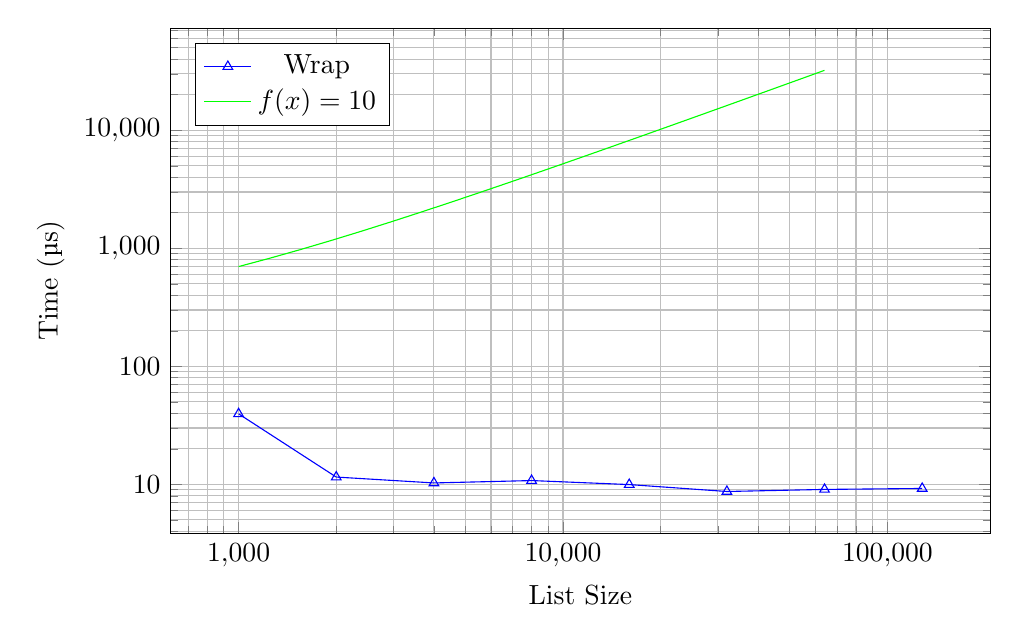
\begin{tikzpicture}
    \begin{axis}[
    xlabel={List Size},
    ylabel={Time (µs)},
    width=12cm,
    height=8cm,
    xmode=log,
    ymode=log,
    grid=both,
    legend pos=north west,
    log ticks with fixed point
    ]
    % Wrap
    \addplot[blue, mark=triangle] coordinates {
    (1000, 39.59)
    (2000, 11.53)
    (4000, 10.28)
    (8000, 10.77)
    (16000, 9.96)
    (32000, 8.70)
    (64000, 9.06)
    (128000, 9.23)
    };
    \addlegendentry{Wrap}

    \addplot[color=green, domain=1000:64000, samples=20] {x/2 + 200};
    \addlegendentry{$f(x) = 10$}
    
    \end{axis}
    \end{tikzpicture}
    \caption{Log-log plot for Wrap queueand the arvage run time per operation for Wrap queue}
    \label{fig:wrap_linked_comparison}
\end{figure}
The analysis reveals that the wrap-around queue maintains consistent performance even as the queue size increases. The average time per operation is approximately 10 nanoseconds, which is better than both the normal and improved linked list-based queue implementations. The best-fit function for the wrap-around queue is $f(x)=10$, indicating constant-time behavior. This confirms the efficiency of the wrap-around technique in managing queue operations.

\section*{Conclusion}
This report has demonstrated the effectiveness of the wrap-around technique in implementing an efficient array-based queue. By reusing space in the array and dynamically resizing it when necessary, the wrap-around queue achieves constant-time performance for both enqueue and dequeue operations, $O(1)$. This represents a significant improvement over traditional array-based queues, which often require $O(n)$ time for certain operations. The wrap-around technique also ensures efficient memory usage, making it suitable for applications where memory is a critical resource.

The dynamic resizing strategy further enhances the queue's scalability, allowing it to handle large numbers of elements without significant performance degradation. While the wrap-around queue introduces some complexity in managing the front and rear indices, the performance gains outweigh this added complexity. Future work could explore additional optimizations, such as more sophisticated resizing strategies or hybrid approaches that combine the benefits of arrays and linked lists.

Overall, the wrap-around queue serves as a valuable example of how careful design choices can lead to significant improvements in both performance and memory efficiency. This implementation highlights the importance of understanding the trade-offs between different data structures and choosing the right approach based on the specific requirements of the application. By mastering techniques like the wrap-around queue, developers can create more efficient and scalable systems, ensuring optimal performance even under demanding conditions.